\documentclass{ibetest}
\begin{document}
\maketest{Progress Test 3.B --- Thermo-S1}
         {3.B \,$\cdot$\, The ideal gas and Clapeyron's law}
         {10 minutes}{14}

% ---------------------------------------------------------------------------
\exercise{Units}{1 mark}
Express the unit of the gas constant $R$, $\mathrm{J\,K^{-1}\,mol^{-1}}$, in SI base units.
\answer{1}{2.2cm}{%
  $1\ \mathrm J = 1\ \mathrm{N\,m} = 1\ \mathrm{kg\,m^2\,s^{-2}}$ \qquad
  $\boxed{[R] = \mathrm{kg\,m^2\,s^{-2}\,K^{-1}\,mol^{-1}}}$}
\begin{scheme}
\pt{1}{1 pt}{$\mathrm{kg\,m^2\,s^{-2}\,K^{-1}\,mol^{-1}}$.}
\end{scheme}

% ---------------------------------------------------------------------------
\exercise{The ideal gas --- definition and Clapeyron's law}{5 marks}
Define the ideal gas model. Write Clapeyron's law, giving the SI unit of every quantity and
the value of $R$.
\answer{2,2,1}{5.8cm}{%
  The \textbf{ideal gas} is the limit model towards which \emph{all} gases tend when their
  particle density $n/V$ is low enough. Its particles have no interactions other than
  collisions with the walls of the container.\\[5pt]
  \textbf{Clapeyron (1834):}\qquad $\boxed{pV = nRT}$\\[4pt]
  $p$ in Pa, \ $V$ in $\mathrm{m^3}$, \ $n$ in mol, \ $T$ in K, \
  $R = 8.314\ \mathrm{J\,K^{-1}\,mol^{-1}}$.}
\begin{scheme}
\pt{1}{2 pts}{Low-density limit (1~pt); no interactions between particles (1~pt).}
\pt{2}{2 pts}{$pV = nRT$.}
\pt{3}{1 pt}{The five units, with $T$ in kelvins, and $R\approx8.31$ SI.}
\end{scheme}

% ---------------------------------------------------------------------------
\exercise{Controlled and free variables}{3 marks}
\question{For a hot-air balloon (opening at the bottom, rigid envelope), the variables held
  fixed are:}
\opts{0}{$n$ and $V$}{1}{$p$ and $V$}{0}{$n$ and $T$}{0}{$n$ and $p$}
\why{Tab.~5: $p = p_{\text{atm}}$ (mechanical equilibrium) and $V$ is fixed by the rigid
  envelope. $n$ and $T$ are free: heating drives air out.}
\question{A weather balloon (sealed, flexible) rises; the outside pressure decreases while its
  temperature stays about the same. Its volume:}
\opts{1}{increases}{0}{decreases}{0}{stays the same}{0}{becomes zero}
\why{$n$ is fixed and $p = p_{\text{atm}}$ decreases. With $pV = nRT$ and $T$ about
  constant, $V$ increases.}
\question{$1.0$~mol of gas at $300$~K and $1.0\times10^{6}$~Pa occupies $2.5$~L. With
  $RT\approx2.5\times10^{3}\ \mathrm{J\,mol^{-1}}$, its compressibility factor
  $Z = pV/(nRT)$ is about:}
\opts{0}{$0.1$}{1}{$1.0$}{0}{$10$}{0}{$2.5$}
\why{$Z = \frac{1.0\times10^{6}\times2.5\times10^{-3}}{2.5\times10^{3}} = 1.0$: the gas
  behaves as an ideal gas. (Compare the worked example of the notes: 1~mol of air in 2~L
  at 2~bar and $25\ ^\circ$C is far from ideal.)}

% ---------------------------------------------------------------------------
\exercise{Piston and cylinder}{5 marks}
\noindent\begin{minipage}[c]{0.58\textwidth}
A horizontal cylinder of cross-section $S$ contains $n$ moles of air, treated as an ideal gas.
The piston is initially at $L_1$ and the temperature is $T_1$.
\end{minipage}\hfill
\begin{minipage}[c]{0.38\textwidth}\centering
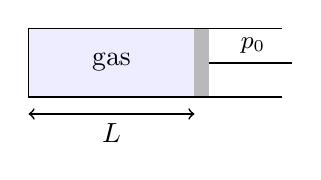
\begin{tikzpicture}[scale=0.62, line width=0.6pt]
  \fill[blue!7] (0,0) rectangle (3.4,1.4);
  \draw (5.2,0) -- (0,0) -- (0,1.4) -- (5.2,1.4);
  \node at (1.7,0.7) {gas};
  \fill[gray!55] (3.4,0.02) rectangle (3.7,1.38);
  \draw (3.7,0.7) -- (5.4,0.7);
  \draw[<->] (0,-0.35) -- (3.4,-0.35) node[midway, below] {$L$};
  \node[font=\small] at (4.6,1.05) {$p_0$};
\end{tikzpicture}
\end{minipage}\\[3pt]
(1) Compute $p_1$. \ (2) The gas is compressed isothermally to $L_2$: compute $p_2$.
\ (3) The piston is locked at $L_2$ and the gas is heated to $T_3$: compute $p_3$.
\ (4) The piston is released against the atmosphere $p_0$, at $T_4 = T_3$: compute $V_4$ and
$L_4$.
\data{$S = \qty{50}{\centi\metre\squared}$ \hspace{7mm} $n = \qty{0.10}{mol}$ \hspace{7mm}
      $L_1 = \qty{50}{cm}$ \hspace{7mm} $L_2 = \qty{25}{cm}$ \hspace{7mm}
      $T_1 = \qty{300}{K}$\\[2pt]
      $T_3 = \qty{450}{K}$ \hspace{7mm} $p_0 = \qty{1.0e5}{Pa}$ \hspace{7mm}
      $RT\approx\qty{2.5e3}{\joule\per\mole}$ at $\qty{300}{K}$}
\answer{1,1,1,1,1}{6.6cm}{%
  (1) $V_1 = SL_1 = 50\times10^{-4}\times0.50 = 2.5\times10^{-3}\ \mathrm{m^3}$ \qquad
  $p_1 = \dfrac{nRT_1}{V_1} = \dfrac{0.10\times2.5\times10^{3}}{2.5\times10^{-3}}$ \qquad
  $\boxed{p_1 = 1.0\times10^{5}\ \mathrm{Pa}}$\\[4pt]
  (2) $n$ and $T$ fixed: $p_1V_1 = p_2V_2$, so $p_2 = p_1\dfrac{L_1}{L_2}$ \qquad
  $\boxed{p_2 = 2.0\times10^{5}\ \mathrm{Pa}}$\\[4pt]
  (3) $n$ and $V$ fixed: $\dfrac{p}{T} = $ const., so $p_3 = p_2\dfrac{T_3}{T_1}
  = 2.0\times10^{5}\times\dfrac{450}{300}$ \qquad $\boxed{p_3 = 3.0\times10^{5}\ \mathrm{Pa}}$\\[4pt]
  (4) $n$, $T$ and $p = p_0$ fixed: $V_4 = \dfrac{nRT_4}{p_0}$, with
  $RT_4 = 1.5\times2.5\times10^{3} = 3.75\times10^{3}\ \mathrm{J\,mol^{-1}}$:\\[3pt]
  \hspace*{5mm}$V_4 = \dfrac{0.10\times3.75\times10^{3}}{1.0\times10^{5}}$ \qquad
  $\boxed{V_4 = 3.75\times10^{-3}\ \mathrm{m^3}}$ \qquad
  $L_4 = \dfrac{V_4}{S} = \dfrac{3.75\times10^{-3}}{5.0\times10^{-3}}$ \qquad
  $\boxed{L_4 = 0.75\ \mathrm m}$}
\begin{scheme}
\pt{1}{1 pt}{$p_1 = 1.0\times10^{5}\ \mathrm{Pa}$ (with $S$ and $L_1$ converted to SI).}
\pt{2}{1 pt}{$p_2 = 2.0\times10^{5}\ \mathrm{Pa}$.}
\pt{3}{1 pt}{$p_3 = 3.0\times10^{5}\ \mathrm{Pa}$.}
\pt{4}{1 pt}{$V_4 = 3.75\times10^{-3}\ \mathrm{m^3}$ (3.75~L).}
\pt{5}{1 pt}{$L_4 = 75$~cm.}
\end{scheme}
\begin{tip}
As in Tab.~5 of the notes, first list which variables are fixed at each step: then the right
law ($pV$, $p/T$ or $V/T$ constant) follows at once.
\end{tip}

\finish
\end{document}
